\documentclass[12pt,a4paper]{article}
\usepackage[utf8]{inputenc}
\usepackage[T1]{fontenc}
\usepackage{amsmath}
\usepackage{textcomp}

\usepackage{geometry}
\geometry{a4paper,left=25mm,right=25mm, top=2cm, bottom=2cm} 

\usepackage{graphicx} %fuer bilder

\usepackage{verbatim}



 \usepackage{mathptmx}
 \usepackage[scaled=.90]{helvet}
 \usepackage{courier}


\usepackage{listings}
\usepackage{color}
 
\definecolor{dkgreen}{rgb}{0,0.6,0}
\definecolor{gray}{rgb}{0.5,0.5,0.5}
\definecolor{mauve}{rgb}{0.58,0,0.82}

\pagestyle{empty}
\lstset{numbers=left,language=C++}
\lstset{showstringspaces=false,
basicstyle=\ttfamily\footnotesize,
breaklines=true,
tabsize=3,
commentstyle=\color{dkgreen},      % comment style
inputencoding={ansinew},
title=\lstname %zeigt titel der datei an
}

\usepackage{pdfpages}% fuer pdfs



%keine einrückungen bei absatz
\parindent 0pt

\begin{document}
\title{Übung 02}
\author{Bernhard Selymes; Reinhard Penn}
\date{April 2013}

\normalsize

%Pfad zu c++ Dateien


%Beginn des Dokuments

\newcommand{\Uebung}{Uebung02}
\newcommand{\path}{../Uebung02}

%Angabe
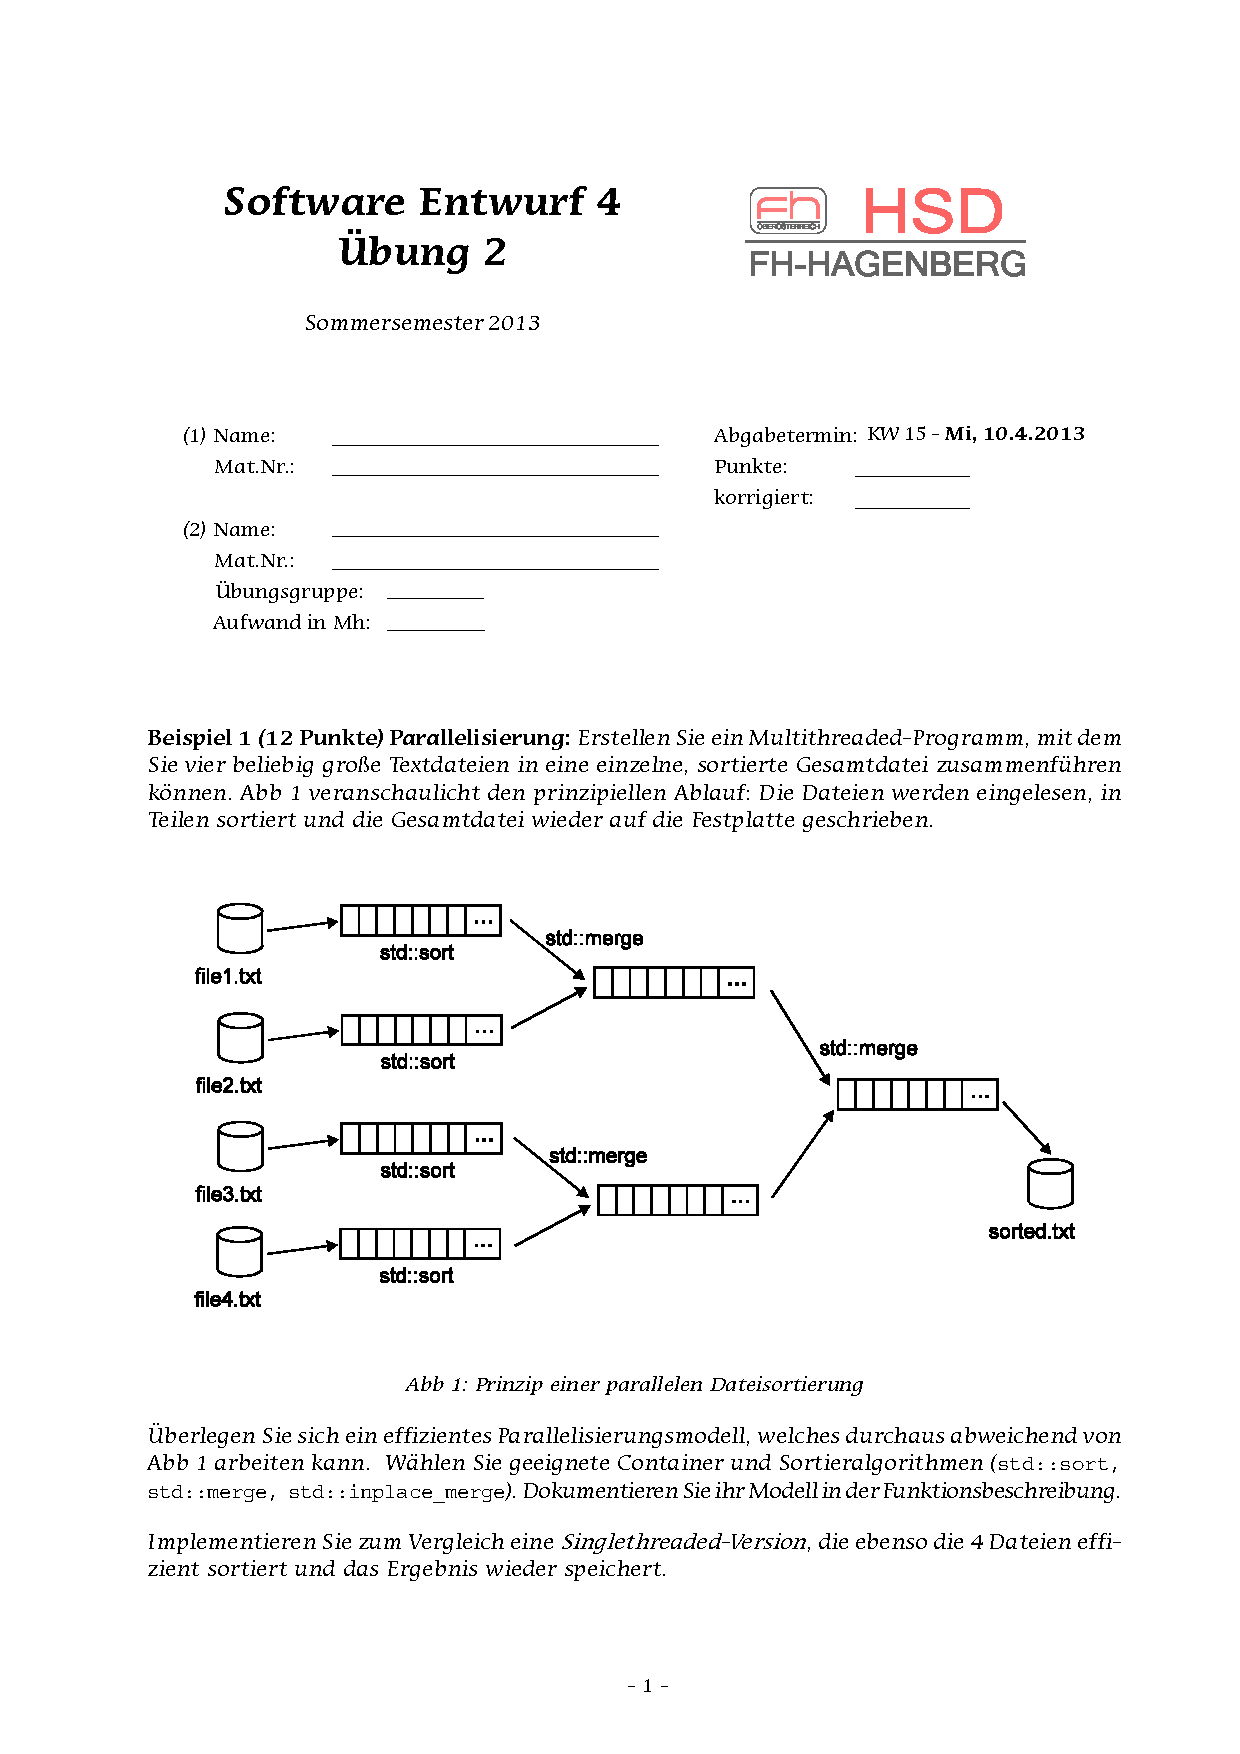
\includepdf[pages=-]{../Angabe.pdf}

\section{Beispiel 1}
\subsection{Funktionsbeschreibung}

Es gibt 4 verschiedene Arten von Workerthreads: 
\begin{itemize}
\item Datei zu Liste
\item Liste zu Datei
\item Liste sortieren
\item 2 Listen zusammenfügen
\end{itemize}
Es gibt für jede Arbeit einen eigenen Thread, dadurch ist die Software übersichtlicher und leichter erweiterbar. Zum Beispiel beliebige Anzahl von Eingangsdateien oder auch Ausgangsdateien. Der Thread der die letzte Liste in die Datei schreibt hätte auch wie die singlethreaded Version implementiert werden können und wäre dadurch auch schneller gewesen. Im Mainthread werden die Handles in Vektoren verwaltet. Von dort werden sie den Threads gegeben. Die Threads warten auf die Threads von denen sie die Handles haben und schließen diese danach.
\newline
Die Daten der Dateien werden in 4 Listen gespeichert. Diese 4 Listen werden sortiert. Danach werden 2 mal 2 Listen zusammengefügt und wieder danach werden die letzten 2 Listen zusammengefügt. Die letzte Liste wird wieder in die Datei geschrieben.
\newline
Anmerkung: Es wurden keine Fehlerfälle im Testtreiber getestet, weil diese  durch Exceptions abgefangen werden würden.
\newline 
Aufgabenaufteilung: Beispiel 1: Bernhard Selymes, Beispiel 2: Reinhard Penn

\subsection{Schnittstellen}
Name: SortMergeMT(...) und SortMergeST(...)
\newline
Parameter: vector<string> const\& filenames, string const\& filenameOutput
\newline
Vektor wegen Erweiterbarkeit und einfacherer Handhabung.
\newline
\newline
\textbf{Schnittstellen der Threads:} Bei der Init Funktion werden jeweils die benötigten Listen und Handles mitgegeben. Die Listen via Pointer, weil sonst die ganze Liste kopiert werden müsste und auch die falsche Liste verändert werden würde. Diese Parameter werden in den Threads jeweils gespeichert.

\subsection{Singlethreaded Version}
Bei dieser Version werden die Daten aller Dateien gleich in eine Liste geschrieben. Diese Liste wird dann sortiert und wieder in eine Datei geschrieben.
\newline
\textbf{Speedup:} 
\newline
Speedup  = 5.885/5.695 = 1.0334
\newline
Die längste Zeit dauert das Schreiben auf die Festplatte.

\newpage
\subsection{Sourcecode}
\lstinputlisting[language={c++}]{\path/Bsp01/StopWatch.h}
\lstinputlisting[language={c++}]{\path/Bsp01/StopWatch.cpp}

\lstinputlisting[language={c++}]{\path/Bsp01/ThreadBase.h}
\lstinputlisting[language={c++}]{\path/Bsp01/ThreadBase.cpp}

\lstinputlisting[language={c++}]{\path/Bsp01/ThreadFileToList.h}
\lstinputlisting[language={c++}]{\path/Bsp01/ThreadFileToList.cpp}

\lstinputlisting[language={c++}]{\path/Bsp01/ThreadListToFile.h}
\lstinputlisting[language={c++}]{\path/Bsp01/ThreadListToFile.cpp}

\lstinputlisting[language={c++}]{\path/Bsp01/ThreadSort.h}
\lstinputlisting[language={c++}]{\path/Bsp01/ThreadSort.cpp}

\lstinputlisting[language={c++}]{\path/Bsp01/ThreadMerge.h}
\lstinputlisting[language={c++}]{\path/Bsp01/ThreadMerge.cpp}

\lstinputlisting[language={c++}]{\path/Bsp01/SortMergeMT.h}
\lstinputlisting[language={c++}]{\path/Bsp01/SortMergeMT.cpp}

\lstinputlisting[language={c++}]{\path/Bsp01/main.cpp}

\lstinputlisting[language={c++}]{\path/Bsp01_SingleThreaded/SortMergeST.h}
\lstinputlisting[language={c++}]{\path/Bsp01_SingleThreaded/SortMergeST.cpp}

\lstinputlisting[language={c++}]{\path/Bsp01_SingleThreaded/main.cpp}

\newpage
\subsection{Testausgabe}
Multithreaded(Release):
\begin {verbatim}
Start timer.
End timer. Time: 5.695
Press a key...
\end {verbatim}

Multithreaded(Debug ohne Ende(dauert ewig)):
\begin {verbatim}
Start timer.
Error in SortMergeMT::SortMergeMT: no valid vector
Error in SortMergeMT::SortMergeMT: no valid string at index 0
Error in SortMergeMT::SortMergeMT: no valid vector
Error in SortMergeMT::SortMergeMT: no valid filenameOutput
\end {verbatim}

Singlethreaded(Release):
\begin {verbatim}
Start timer.
End timer. Time: 5.885
Press a key...
\end {verbatim}

Singlethreaded(Debug ohne Ende(dauert ewig)):
\begin {verbatim}
Start timer.
Error in SortMergeST::SortMergeST: no valid vector
Error in SortMergeST::SortMergeST: no valid string at index 0
Error in SortMergeST::SortMergeST: no valid vector
Error in SortMergeST::SortMergeST: no valid filenameOutput
\end {verbatim}

\newpage
\section{Beispiel 2}

\subsection{Funktionsbeschreibung}
Das AdminTool besteht aus einer Klasse die nur statische Funktionen enthält. Die Funktionen wurden statisch erstellt, da die Funktionalität des AdminTools nicht vom jeweiligen Objekt abhängig ist. Das AdminTool kann Prozesse starten und beenden. Zum Prozess starten muss der jeweilige Name des Programms übergeben werden, zum beenden wird die Prozess-Id übergeben. Eine weitere Funktion des AdminTools ist es alle laufenden Prozesse aufzulisten. Dabei wird Prozessname, ProzessId, BasePriority und ThreadCount ausgegeben. Die letzte Funktion des AdminTools ist es Systeminformationen auszugeben. Zum Beispiel: Prozessorarchitektur, Anzahl der Prozessorkerne, Computername, OS-Version,... . Die Fehlerbehandlung erfolgt mittels Exception die im Testtreiber abgefangen werden. Im Testtreiber wird ein einfaches Menü zur Verwaltung der Funktionen des AdminTools erzeugt.
\newline
\newline
\textbf{Schnittstelle:}
\newline
Name: StartProgram
\newline
Returnwert: void
\newline
Parameter: 
\newline
size\_t ProgramName: Name des zu startenden Programms
\newline
\newline
Name: ListProcesses
\newline
Returnwert: void
\newline
\newline
Name: KillProcess
\newline
Returnwert: void
\newline
Parameter: 
\newline
size\_t ProcessId: Prozess Id, des Prozesses der terminiert wird
\newline
\newline
Name: PrintSystemInfo
\newline
Returnwert: void
\newline




\newpage
\subsection{Sourcecode}
\lstinputlisting[language={c++}]{\path/../PSS4_UE02_AdminTool/PSS4_UE02_AdminTool/AdminTool.h}
\newpage
\lstinputlisting[language={c++}]{\path/../PSS4_UE02_AdminTool/PSS4_UE02_AdminTool/AdminTool.cpp}
\newpage
\lstinputlisting[language={c++}]{\path/../PSS4_UE02_AdminTool/PSS4_UE02_AdminTool/main.cpp}

\newpage
\subsection{Testausgabe}

\begin{verbatim}
Enter command: ?
StartProgram: 0
ListProcesses: 1
Remove: 2
KillProcess: 3
PrintSystemInfo: 4
Exit: e

Enter command: 0
Enter program name: not_existing
CreateProcess failed: Das System kann die angegebene Datei nicht finden.

Enter command: 0
Enter program name: notepad

Enter command: 1
Process                  PID       BasePriority        Thread Count
----------------------------------------------------------------------
[System Process]         0         0                   4
System                   4         8                   114
smss.exe                 296       11                  3
csrss.exe                392       13                  9
wininit.exe              464       13                  3
csrss.exe                492       13                  13
services.exe             524       9                   7
lsass.exe                540       9                   8
lsm.exe                  548       8                   10
svchost.exe              656       8                   10
svchost.exe              740       8                   8
atiesrxx.exe             800       8                   6
winlogon.exe             848       13                  3
svchost.exe              900       8                   23
svchost.exe              932       8                   34
svchost.exe              972       8                   21
svchost.exe              1008      8                   39
UMVPFSrv.exe             324       8                   3
svchost.exe              1124      8                   16
atieclxx.exe             1228      8                   10
spoolsv.exe              1396      8                   13
sched.exe                1424      8                   7
svchost.exe              1448      8                   19
armsvc.exe               1564      8                   4
Fuel.Service.exe         1588      8                   6
avguard.exe              1612      8                   35
bitkinexsvc.exe          1648      8                   4
jtagserver.exe           1736      8                   4
sqlservr.exe             1760      8                   35
mysqld.exe               1780      8                   22
sqlwriter.exe            1928      8                   4
TeamViewer_Service.exe   1104      8                   6
VC9SecS.exe              1496      8                   5
WLIDSVC.EXE              960       8                   8
WLIDSVCM.EXE             2272      8                   3
avshadow.exe             2660      8                   3
conhost.exe              2668      8                   1
avwebgrd.exe             2700      8                   10
SearchIndexer.exe        2808      8                   13
svchost.exe              2960      8                   16
wmpnetwk.exe             2984      8                   13
svchost.exe              2540      8                   26
dwm.exe                  1952      13                  5
explorer.exe             3008      8                   25
ddm.exe                  3384      8                   9
avgnt.exe                3708      8                   11
acrotray.exe             3808      8                   2
MOM.exe                  3876      8                   15
svchost.exe              3436      8                   6
CCC.exe                  5084      8                   27
svchost.exe              5636      8                   11
dllhost.exe              5344      8                   5
PresentationFontCache.exe4128      8                   6
texmaker.exe             6796      8                   4
devenv.exe               7896      8                   26
vcpkgsrv.exe             6092      8                   5
mspdbsrv.exe             3868      8                   3
wuauclt.exe              4056      8                   3
MpCmdRun.exe             6440      8                   8
vcpkgsrv.exe             1696      8                   8
cmd.exe                  7760      8                   1
conhost.exe              3884      8                   2
PSS4_UE02_AdminTool.exe  7964      8                   1
notepad.exe              6640      8                   1

Enter command: 2
Enter process Id of process to kill: 123123123
OpenProcess failed: Falscher Parameter.

Enter command: 2
Enter process Id of process to kill: 0
OpenProcess failed: Falscher Parameter.

Enter command: 2
Enter process Id of process to kill: 4
OpenProcess failed: Zugriff verweigert

Enter command: 2
Enter process Id of process to kill: 6640

Enter command: 3
System Information <HARDWARE>:
------------------------------
Processor Type           : 586
Architecture             : Intel CPU or compatibles
Processor Level (Family) : 16
Model and Stepping MMSS  : 0x402
Number of Processors     : 4


System Information <SOFTWARE>:
------------------------------
Computer Name: REINHARD-PC
OS Version   : Major: 6  Minor: 1
OS Revision  : Service Pack 1

Enter command: e
Drücken Sie eine beliebige Taste . . .
\end{verbatim}


\end{document}
